\documentclass{article}
\usepackage[utf8]{inputenc}
\usepackage[right=2cm,left=3cm,top=2cm,headsep=0.5cm,footskip=0.5cm]{geometry}

\title{The Impossible  Early Galaxy Problem}
\author{Santiago Arranz Sanz }
\date{June 2019}

\usepackage{natbib}
\usepackage{graphicx}
\usepackage{latexsym}
\usepackage{eufrak}
\usepackage{dsfont}
\usepackage{hyperref}
\usepackage{enumerate} 
\usepackage{lscape}
\usepackage{titlesec}
\usepackage{fancyhdr}
\usepackage{color}


\newtheorem{teo}{\underline{Teorema}}
\newtheorem{defi}{\underline{Definici\'on}}
\newtheorem{propo}{\underline{Proposici\'on}}
\newtheorem{ejem}{\underline{Ejemplo}}[section]
\newtheorem{prob}{\underline{Problema}}
\newtheorem{lema}{\underline{Lema}}
\newtheorem{obs}{\underline{Observaci\'on}}
\newtheorem{ide}{\underline{Idea}}

\begin{document}

\maketitle

\section*{Introduccion}

Después de leer varios artículos en los que trata dicho problema y derivados he llegado a la conclusión que el problema base es la discordancia del modelo actual de fusión jerárquica con la falta de observación de galaxias transitorias entre los halos iniciales y las galaxias más masivas en los redshift $z\sim 4-6$. Veamos algunos resumenes de los artículos principales.

\section*{The Impossible Early Galaxy Problem}
\citep{steinhardt2016impossibly} Según el paradigma actual de la fusión jerárquica de galaxias en el modelo cosmológico estandar, en torno a los redshift $z\sim 4-6$ ha de existir la transición de las galaxias más masivas desde los halos iniciales que acretan masa a las últimas fases de evolución bariónica vista en las galaxias con formación estelar y \textit{quasars}. Sin embargo, ninguna evidencia ha sido encontrada en muchos estudios a alto redshift como el CFHTLS, CANDELS y el SPLASH, los primeros estudios para probar la masa alta final en estos redshift. Considerando que el ratio masa estelar- masa halo (SMHMR) estimado a bajo redshift permaneciera constante en $z\sim 6-8$, CANDELS y SPLASH darían mayores ordenes de magnitud de número de halos de masa $M\sim 10^{12-13}M_\odot$ que los que se podrían haber formado a esos redshift, esto se conoce como el problema de la galaxia masiva temprana imposible. En el artículo de \cite{steinhardt2016impossibly} consideran los posibles errores sistemáticos que puedan explicar esta contradicción de teoría y observaciones en los modelos de síntesis estelar usados para estimar los parámetros físicos  y en los escenarios posibles de formación galáctica. Es posible que las incertidumbres desconocidas reduzcan la disparidad entre observaciones y simulaciones de CMD tomando una visión conservadora de las observaciones,aun así existirían tensiones considerables con la teoría.\\

Existe un consenso bastante amplio en la distribución de masa y redshift de los halos producidos en el colapso inicial de las pequeñas fluctuaciones de densidad en el universo temprano y el modelo de fusión jerárquico. Para la cosmología estándar la función de masa es sencilla de calcular. Este consenso se basa en la idea de la rápida evolución en la densidad de halos masivos en $z>4$ que deberían ser observacionalmente evidente en las funciones de masa y luminosidad galácticas. Hasta hace poco el catálogo de galaxias a redshift $z>6$ era limitado y sesgado a las galaxias más brillantes, galaxias individuales masivas y \textit{quasars}. Sin embargo con los nuevos estudios como el CANDELS o el SPLASH se ha podido probar la función de luminosidad y de masa para galaxias en el rango de $z\sim 4-8$, lo que nos permite calcular la función de masa del halo correspondiente a dicho rango.\\

Trabajos como el de \cite{finkelstein2015increasing} muestra las tensiones ocasionadas en $z>4$ entre la evolución esperada de la función de masa del halo y las funciones de luminosidad y de masa de las galaxias.\footnote{El resumen de dicho trabajo lo podemos encontrar en \cite{arranz2015finkelstein}} \\

\section*{Galaxias tempranas y sus halos}
Como hemos visto en el trabajo de \cite{finkelstein2015increasing} la teoría espera una rápida evolución en las galaxias entre los redshift de $z=4-7$, sin embargo las observaciones no avalarón dichas prediccionas en su trabajo. En el trabajo de \cite{steinhardt2016impossibly} pretende extender y actualizar los resultados de trabajos como el de \cite{finkelstein2015increasing} basándose en los datos de CANDELS y SPLASH. La ventaja de tomar redshift altos como los del estudio de $z=4-8$ es que tenemos un tiempo cósmico más pequeños (0.9 Gyr \citep{steinhardt2016impossibly}) en un mayor número de redshift, lo que debiese permitir ver una evolución mas detallada que en redshift bajos. Por otro lado los métodos de estimación de las masas de los halos son menos abundantes por lo que el trabajo de \cite{steinhardt2016impossibly} trabaja básicamente con tres tipos de estimaciones.
\begin{enumerate}
\item El primero de ellos se base en la clusterización \citep{hildebrandt2009cars} el cual estima la masa del halo según la distribución espacial de las galaxias. La ventaja de este método es que no hay que asumir ninguna propiedad física de las galaxias, pero sí es necesario escoger un modelo de materia oscura para las simulaciones.
\item Un segundo método es el presentado y desarrollado en el artículo de \cite{finkelstein2015increasing}, el cual se basa en la curva de luminosidad UV \footnote{Hay que recordar que podría ser incorrecta ya que en el artículo de se asumio la existencia de galaxias solo visibles en submilimétricas \citep{wang2019dominant}.} y en la función de masa calculada a través de simulaciones, relacionando ambas por el principio de que el halo más masivo a de albergar la galaxia más masiva y viceversa.
\item El último método es asumir un ratio entre luminosidad/masa estelar y materia oscura. El ratio asumido es el redshift más bajos donde las estimaciones de materia oscura son más factibles por los métodos de agrupación. El ratio usado para el enlace entre masa estelar y de halo es  $M_h/M_\star \sim 70 $.
\end{enumerate}

\textcolor{red}{Sobre el primer método no puedo decir mucho de momento ya que no he leido el paper de \cite{hildebrandt2009cars} donde desarrollan el método, pero al igual que en el último método depende de un modelo de materia oscura lo cual podría ser una variable a tener en cuenta para que los resultados cuadren con las observaciones. Sobre el segundo método ya se ha discutido los posibles fallos en \cite{arranz2015finkelstein} que puede tener sobre todo a raiz del descubrimiento de \cite{wang2019dominant}. Por último considera un ratio igual a redshift más bajos lo cual no tendría porque ser cierto si las propiedades de galaxias y halos evolucionan con el tiempo, lo que podría demostrar el artículo de \cite{wang2019dominant} contradiciendo las suposiciones realizadas en \cite{finkelstein2015increasing}. Todos estos puntos débiles pueden ser clave fundamental para poner en duda dichos resultados.}\\

\begin{figure}[h]
\begin{center}
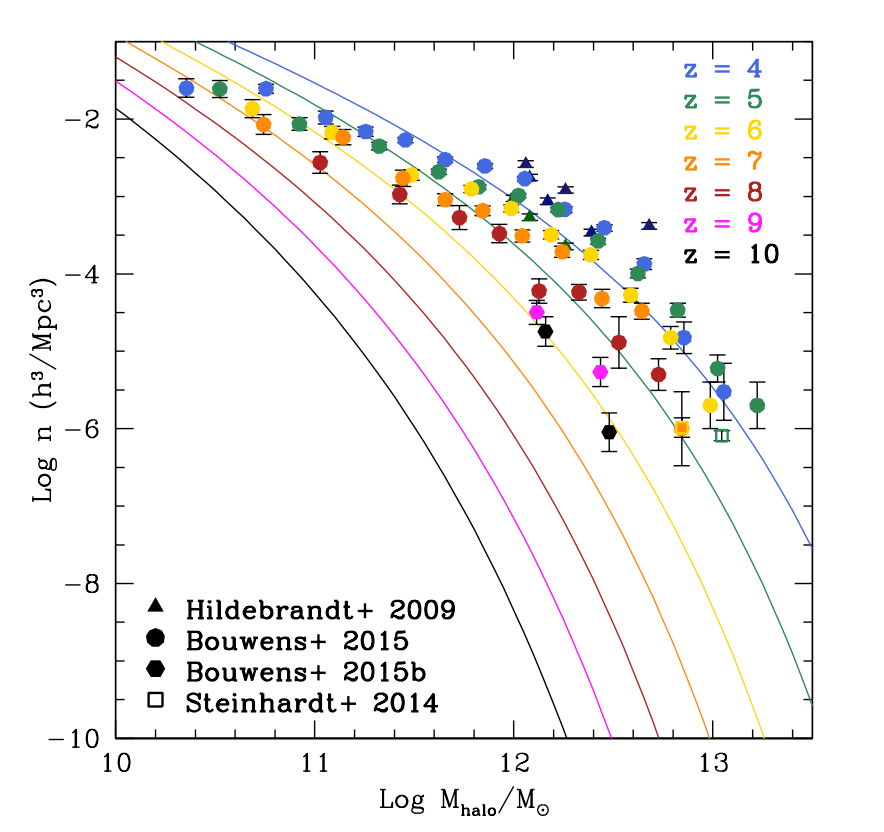
\includegraphics[scale=0.55]{Figuras/steindhart_fig1.png}
\caption{\label{fig:steindhart_fig1} Imagen que representa las estimaciones teoricas del número de densidad de halos en función de su masa versus las obtenidas de las observaciones estudiadas en \cite{steinhardt2016impossibly}}
\end{center}
\end{figure}

Las estimaciones teóricas de la función de masa de los halos para los diferentes redshift han sido sacadas de la herramienta \cite{murray2013hmfcalc} la cual esta basada en el trabajo \cite{sheth2001ellipsoidal}. Las discrepancias que se pueden observar en la \textbf{Figura \ref{fig:steindhart_fig1}} son muy visibles, en especial se encuentran la función de masa del halo de las observaciones tienen un mayor número de densidad de halos masivos con respecto a los predichos por la teoría. Una posible explicación es que el ratio $M_h/L_{UV}$ en galaxias masivas decrece bruscamente en $z>4$, tendiendo a sobrestimar la masa de halos de las galaxias de alto redshift. Si esto fuera así se podría esperar que esta rápida evolución tuviera que ser evidente en otras propiedades medibles de la población de galaxias. En el siguiente punto del artículo de \cite{steinhardt2016impossibly} trata esta posibilidad sin encontrar ninguna evidencia de dicha evolución del ratio de masa halo y luminosidad. \textcolor{red}{Esta posibilidad solo explicaría las medidas basadas en luminosidad, quedando fuera quizás el primer método de clusterización. Por otro lado, la evolución drástica en luminosidad podría hacer que no se viesen todas las galaxias del halo \citep{wang2019dominant} por lo que afectaría a las medidas basadas en clusterización del primer método}

\section*{Aspecto normal de las galaxias en alto redshift}

\newpage
\bibliographystyle{plainnat}
\bibliography{references}

\newpage
\appendix
\section*{Planteamientos iniciales de cada día de trabajo}
Notas que pretenden estructurar el trabajo día a día
\subsection*{Agosto 2019}
A falta de terminar de analizar el paper de \cite{finkelstein2015increasing} y de hacer una lista de las dudas surgidas y propuestas a dar ya he leido el artículo de \cite{wang2019dominant} sobre las galaxias a redshift $z>3$ descubiertas por ALMA las cuales parecen ser abundantes y masivas y no detectables por el HST. Esto tumbaría la susposición de \cite{finkelstein2015increasing} de la no existencia o poca abundancia de las galaxías sub-milimétricas lo que modificaría la función de luminosidad y por tanto la relación de masa halo - masa estelar ya que en el paper de \cite{finkelstein2015increasing} se basa principalmente en ella. La propuesta de lo que quiero hacer hoy es lo siguiente:
\begin{enumerate}
\item Terminar el análisis de \cite{finkelstein2015increasing}. $\surd$
\item Como encaja las nuevas observaciones de \cite{wang2019dominant} en el paper de \cite{finkelstein2015increasing} $\surd$
\item Plantear como incluir los planteamientos de \cite{wang2019dominant}: 
\begin{enumerate}[i.]
\item Replantear la función de luminosidad de \cite{finkelstein2015increasing}.
\item Como encaja en el modelo jerárquico \citep{bower2006breaking}.
\item Las simulaciones de RAMSES nos pueden dar un orden distinto a la masa de los halos que encajen de una manera distinta de con la función de luminosidad. 
\end{enumerate}
\end{enumerate}

\subsection*{Septiembre 2019}
\subsubsection*{Semana 2: 9-15}
El artículo de \cite{wang2019dominant} parece indicar que algunas de las suposiciones en las que se basan los métodos de cálculo de las masa de halo están equivocados, por lo que el escenario más factible para la resolución del problema de \cite{steinhardt2016impossibly} sea el error observacional. Las tareas para esta semana son las siguientes:
\begin{enumerate}
\item Terminar el análisis de \cite{steinhardt2016impossibly}.
\item Leer el artículo de \cite{sheth2001ellipsoidal} y \cite{murray2013hmfcalc} que trata las estimaciones teóricas usadas para el cálculo de la función de masa de halo. Empezar con el resumen de \cite{sheth2001ellipsoidal}.
\item Terminar el punto 3 de agosto.
\item Escribir a Santi con los avances el domingo día 15 y plantear con él una reunión.
\end{enumerate}
\end{document}
